% !Mode:: "TeX:UTF-8" 
\section{国内外在该方向的研究现状及分析}
\subsection{国外研究现状}

“不确定性”和“服务风险评估”在学术领域是比较关注的问题,研究从建模、对策和软件实施三个层面进行,其中针对对策的研究可分为服务替换~(Web Service substitution)~、故障恢复~(fault recovery)~、服务自愈~(self-healing)~和动态组合~(Dynamic composition)~四类研究方法,思路如图~\ref{uc_ways}~所示。

\begin{figure}[htbp]
\centering
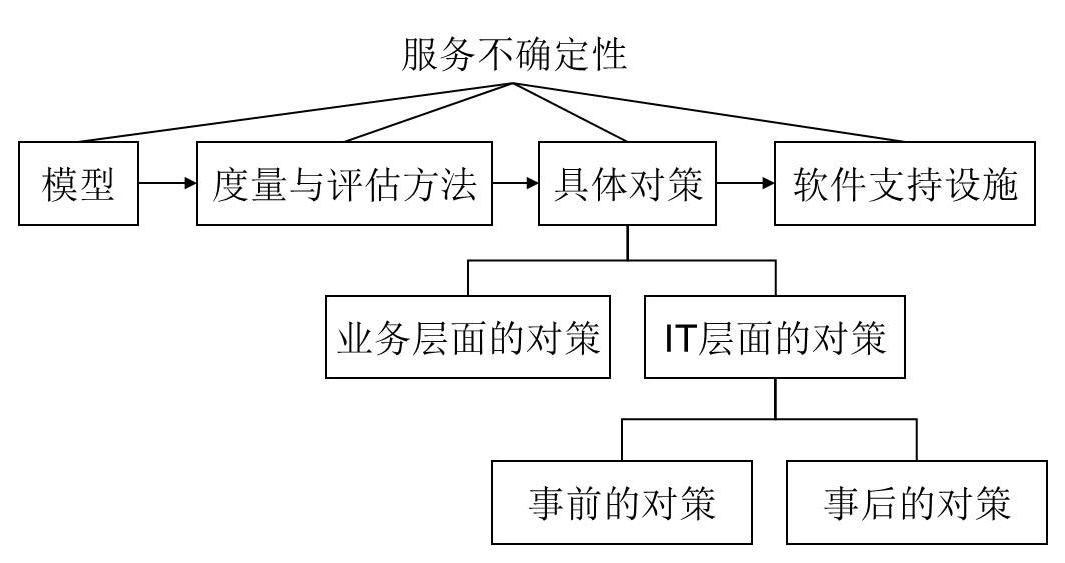
\includegraphics[width = 0.5\textwidth]{uc_ways}
\caption{国内外研究现状综述的线索}\label{uc_ways}
\vspace{-1em}
\end{figure}

根据这个思路,国外的研究现状如下几个方面。

\setcounter{paragraph}{0}
\paragraph{服务风险建模}

在一个服务环境中,用户对服务的使用,需要对服务的~QoS~参数进行定量度量和参数监测,及时检查约定的服务级别和在~SLA~管理中汇报给有关参与者。文献\cite{keller2003wsla}中,介绍了~Web Service Level Agreement (WSLA)~框架,旨在定义和监测~web~服务的~SLA~,标准的~WSLA~框架基于~XML Schema~定义,其灵活和可扩展的描述语言和可以监控不同~SLA~的运行时体系架构。

针对服务运行时可能发生的不确定性(风险),目前的研究从不同角度进行分类和建模。文献\cite{kokash2007evaluating}将其分为服务/数据/用户缺失、非期望的服务行为、性能问题、协议违反等类型。文献\cite{chan2009fault}从物理~(physical)~、开发~(development)~、交互~(interaction)~三个方面将服务的故障分为~13~个小类别,并对其原因和影响进行了全面的分析。文献针对~web~应用层面、~web service~层面、基础设施和中间件层面对可能的服务执行故障分为~9~类,例如~QoS~违反、~WS~执行失败、~WS~协调错误、网络错误等\citeup{ardagna2006faults}。

针对服务的度量建模,相关研究有基于~SLA~的服务风险度量与估算方法\citeup{michalk2010risk}、面向~SLA~一致性分析的自动化算法\citeup{yang2003compatibility}等,以协助客户/提供者发现不确定性以及造成的影响。

\paragraph{不确定性对策}

在前人的研究中,有针对确定的服务不确定性进行了研究,这其中有服务替换、服务故障恢复和服务动态组合等策略。

~a)~服务替换

服务替换是指用一个服务构件替换另一个服务构件,并且替换的构建和被替换的构件具有相同的输入输出,以及相同的需求约束。目前大体上有“接口匹配”、“添加中间件或适配器”、“服务共同体”,它们分别是:

接口匹配的方法,如文献\cite{ponnekanti2004interoperability}提出在以~XML~(主要指~WSDL)描述的~Web Service~中,当一个服务不可用或者出现其他故障时,能够扩展其他基于这个服务的并且具有同样功能的服务,来替换掉出现故障的服务。扩展接口体现在针对于~WSDL~描述的服务接口,增加或者删除某些操作,来扩展或者限制输入和输出消息类型,以满足被替换服务所需求的接口要求。文献\cite{benatallah2005temporal}提出一个绑定于同步业务协议之上的服务是否能不另一个服务替换的方法。文献\cite{salas2006ws}\cite{guo2007angel}也是同样的方法,建立一个能够满足替换要求的候选服务集,一旦服务执行出现故障即用候选服务进行替换。

添加中间件或适配器的方法,也是为了处理替换服务和被替换服务接口之间的不兼容问题。如文献\cite{chen2008web} 在服务组合和适配器之间加一层替换层,使得替换策略灵活和有效的适应组合服务的执行。它的一般步骤是:~(1)~对候选服务进行分组,每一组内的服务可以相互替换;~(2)~在组合服务设计阶段进行静态替换,替换不可用服务;~(3)~服务执行期间,某服务发生不可用/与其他服务冲突/用户需求~QoS~变化,执行动态替换。于此同时,适配器还帮助用户重新完善服务描述,动态适配器在组合阶段或在执行阶段通过封装服务,把接口不匹配的服务转换为接口匹配的服务。

服务共同体~(community)~的方法,文献\cite{medjahed2005dynamic}提出服务共同体的概念,并给出~Web~服务共同体的模板,同时给出其他环境一对一转换到服务共同体的方法。文献\cite{taher2006towards}提出基于服务共同体的在~Open Service Connectivity~构件之上建立服务替换方法,并添加适配器转换规则。它分两步执行替换动作:~(1)~聚集功能相同或相似的~Web~服务到~Communities~中;~(2)~基于~Open Service Connectivity~驱动方法使客户端连接到~Communities。~

~b)~服务故障恢复

当服务出现故障,如何恢复也成为一个研究热点。目前大体上有“错误回滚”、“扩展现有系统”、“提前添加恢复措施”等方法。

错误回滚的方法,如文献\cite{yu2010fault} 提出了一种考虑了事务机制、~QoS~因素、全局限制因素、局部限制因素的容错策略来提高服务组合可靠性,保证服务不出错或者出错能回滚到上一稳定的状态,~Petri~网络的采用使方法更加高效。文献\cite{fan2011approach} 使用
~Petri~网对服务组合的不同组件建模并将面向切面的方法被融入到错误恢复考虑因素。使用的面向切面的方法通过把需要失败恢复的服务组合划分成为单独的切面,并通过~Petri~网增加语义制约来消除面向切面的描述不清等负面影响。

扩展现有系统的方法,如文献\cite{cabrera2002web}提出~Web Service~层面的协调恢复机制,文献\cite{jeckle2003active}提出利用~SOAP~的优点扩展~UDDI~构造了一个~FT-SOAP~系统,使得服务在失败时具有更强的恢复力。

提前添加恢复措施的方法,如文献\cite{erradi2006recovery}提出一系列扩展恢复措施来处理服务执行时可能遇到的错误,它在服务组合阶段完成,因此使得组合服务具有更好的容错性。文献\cite{issarny2003coordinated}提出一种~Web Service~环境下支持可靠系统的发展,也使得组合服务具有更强的可靠性。

~c)~服务动态组合

根据服务流程的执行结果来执行动态组合,指在组合服务执行了一段时间之后,采用目前的执行结果,动态组合出新的服务组合流程,以满足服务能够最终执行成功。目前大致有“影响范围最小化”、“人工智能”等方法。

影响范围最小化的方法,如文献\cite{yin2009self}介绍了一种自治愈的~Web~服务组合模型,是一种支持补偿的综合客观~QoS~驱动的服务替换模型,这个模型的关键是确定并最小化影响的范围:找出不可用服务、找出最小关联范围和找出最小替换范围。文献\cite{li2011adaptive}提出自适应~QoS~感知服务过程的重构,它提出的服务组合方法是在服务组合过程中选择一些候选服务作为高效恢复的一种备份,通过确定一个包括最少服务的有限重构区域,基于区域的重构算法以尽量降低重构花销。文献\cite{lin2009efficient}提出将服务划分成满足QoS的最小重构区域,对区域内服务进行重构,以最大限度的降低计算复杂度,提高重构效率。

文献\cite{madhusudan2006declarative}提出一种减轻动态服务组合复杂度并可升级的基于~AI~的“集成服务计划与执行”~(Integrated Service Planning and Execution (ISP~\&~E)),并采用~HTN~(Hierarchical Task Network)~网络实现。

\paragraph{软件实施}

在对服务不确定性进行建模和采取决策动作的理论研究之后,需要将具体的方法应用到实际的软件服务中,因此,相关研究包括服务的运行时监控。

基于~SLA~监听的研究,如文献\cite{goel2011sla}提出叫~SLA~监听器的集成系统,形式化的定义了多种~SLA~属性。使得在实际业务流程中,~BLA~(Business Level Agreements)~和~BLO~(Business Level Objectives)~都得到满足。文献\cite{raimondi2008efficient}提出~Web Service~层面的时间自动机来监听服务提供者和用户之间的SLA属性,主要针对延时~(Latency)~、可靠性~(Reliability)~和吞吐量~(Throughput)~。在服务保障的研究中,如文献\cite{bravetti2007theory}\cite{bravetti2009theory}提出在服务组合时对服务进行过滤,使得服务在任何时候调用时都已经就绪,尽可能提高服务可靠度。

在运行时的监控,监听组合服务在执行时的状态,一旦出现故障需要立刻抛出异常并处理。文献\cite{chen2008dynamic}提出~MANET~自组网络的工作组~(Mobile Ad-hoc NETworks)~,针对分布式服务组合执行网络,提出了一种监测服务执行状态的机制,每个执行中的服务的监视器就是他是前驱服务,提供了出错时较高的响应速度。文献\cite{moser2008non}提出了~VieDAME~系统,允许监听~BPEL~流程和监听服务的~QoS~,并能根据一系列的替换策略进行服务替换而不影响~BPEL~的正常执行。文献\cite{baresi2005dynamo}提出一种动态监督框架,扩展~Active BPEL~使得其可以在现有的BPEL执行引擎中执行。

%在软件层面,可采用可靠性保障的方法来解决~web~服务中的不确定性问题\citeup{subramanian2008enhancement},在最初构建服务方案时就考虑可能面临的风险,将可靠性、不确定性等因素加入到服务选择与服务组合模型/算法中,以降低未来执行中的风险。可使用~Stochastic Petri Nets~等工具对~Web~服务组合方案进行建模,以计算组合服务的~reliability\citeup{zhong2008reliability}~,或者考虑服务发生风险时的依赖关系\citeup{liu2009risk},以此作为服务组合的可靠性优化依据,进而通过~Markov~决策过程~(MDP)~等方法来选择最符合客户风险偏好的可靠服务\citeup{harney2008selective}\citeup{gao2011reliability}。
%
%在软件层面,软件服务的不确定性与其可靠性息息相关。软件可靠性领域通常利用基于概率统计的不确定理论对软件可靠性进行建模,通过对软件故障过程分析和相应处理\citeup{zhangyongqiang2006},因此,为了在服务执行产生不确定事件时能够通过恢复机制来保障可靠性\citeup{chan2009design},可基于冗余策略预先配置备用服务或多个替代配置方案(配置树、执行计划)来提升服务方案的容错能力\citeup{kokash2006service},目标是使服务方案具备自我治愈的能力\citeup{ardagna2006faults}。当现有服务无法正常执行时直接由备选服务接替执行,也可采用备选流程的方式,在当前流程出现问题时直接切换到备选流程。为此需在服务建模阶段考虑各种不确定性,对建模元素的实现机制和应用场景进行扩展以提高模型描述能力和适应性\citeup{fan2002service}。
%
%除此之外,~Web~服务过程中的不确定性也可以用补偿流程的方式来处理\citeup{fensel2002web},即:当执行中出现可预料的不确定性时可以按预先指定的流程执行相应的补偿操作从而使服务达到预期的解决效果。这些研究的目标是使服务方案逐渐具备越来越高的自我治愈~(self-healing)~的能力\citeup{ardagna2006faults}。
%
%(4)~IT~层面的不确定性处理对策:事后
%
%虽然SOA提供了一种通过规范说明和发布、发现、选择及组装独立开发的软件组件来构造复杂分布式系统的方法,由于服务环境各方面因素的不确定性,导致在执行过程中可能出现计划服务不可用的情况。在这种情况下,目前研究分别采用服务替换、服务重组等服务重配置方法、恢复与补偿机制等策略来应用执行中可能出现的不确定性\citeup{erradi2006recovery}。
%
%服务替换是指当某个服务不可用时,如何用其他服务替代以维持整个服务过程的完整性和有效性\citeup{li2011petri}\citeup{athanasopoulos2009service}。服务的替换主要考虑服务的功能和非功能特性(主要是质量特性)。功能方面主要基于服务的参数类型等静态属性和动态行为特性\citeup{bordeaux2005two}的匹配保证替换前后服务过程功能的一致性,而非功能方面主要基于客户在QoS偏好对服务效用进行度量来保证和优化替换后的服务质量\citeup{claro2005selecting}。此外还有基于context的手段\citeup{pathak2007context}对服务的可替换性进行判断。
%
%服务重组是指服务过程的重新组合。根据重组方式的不同,可以分为服务的大规模重选取和服务路径的重规划。服务重选取通常是大规模进行的,而服务路径的重规划是指将服务的全部或者部分流程进行重新规划,根据执行过程中所发生的不确定性的种类和严重程度而形成新的执行路径,服务的重规划通常包含了对于服务的重选取。文献\cite{bouhini2010discovery}使用服务片段作为重规划的基本单元以提升效率。文献\cite{bucchiarone2010design}提出了一组系统化的原则和指南,指导设计者如何构造/重规划适应变化的服务。
%
%根据服务重组范围的不同,可以分为服务的完全重组和部分重组两种。完全重组是指在服务执行过程中出现不确定性时,有必要时将撤销或者作废服务过程中的已执行部分,而对整个服务过程进行重规划或者重选取,其代价至少为全新服务组合的代价,因此常常采用部分重组,即针对不同具体情况对服务过程中的部分环节或者子过程进行重规划或者重选取,使得调整后的结果能够满足预期的约束目标。当具体不确定性发生时,服务提供者通常期望以最小代价的改动使得服务过程恢复到满足期望的状态。因此常用的方法是对服务过程中处于不同执行阶段的部分进行划分,并在每次尝试失败后逐渐扩大考虑的范围,每次尝试中都期望在尽量小的范围内弥补甚至消失不确定性产生的后果\citeup{zhai2009soa}。还可使用修补技术对当前服务组合方案进行改变和增强,使之适应各类故障\citeup{yan2010self}。另外,可根据服务执行反馈的状况,采用进行持续规划~(continual planning)\citeup{kaldeli2011continual}~,以适应执行过程中出现的各类不确定情况。


\subsection{国内研究现状}
采用马尔可夫决策过程,如文献[28]提出预见性的服务自愈功能,对服务的替换动作由顾客(客户端)决定,通过观察服务性能,决定是在服务失败前替换还是替换服务构件(重组服务),目标使得替换动作的消耗最小。文章采用马尔可夫决策过程,当在某状态上某服务的QoS变化,决策出最优动作。因为只知道当前的状态,因此决策过程是具有预见性的服务自愈和服务动态组合。文献[33]也采用马尔可夫决策过程来解决服务动态组合问题。


\subsection{国内外文献综述的简析}
如上所述,目前关于服务不确定性的研究已经有了丰富的研究,但尚显不足。

(1)~大部分研究者站在软件服务的开发、运行和维护的角度上,探讨“当某服务执行出现异常”之前或之后如何应对。而本课题站在客户或者中介方的角度,他们作为服务的使用者,不可能也无需了解软件服务的内部执行细节,只是从外部观测到各类异常的发生,而无法得知造成异常的原因(例如服务器内部出错、网络出错等)。在这种情况下,通过各类不确定性的决策方法,提高第三方服务中介所构造的整体服务方案适应不确定性的能力,是本课题的研究重点,也是区别于传统研究的观点之一。

此类问题归纳起来,目前研究主要分为两类:
a)~建模阶段对服务模型进行抗风险能力的增强,一旦运行时发现问题即可按预案进行应对;
b)~运行阶段对相关服务进行替换、重组或修补,并确保操作前后服务功能和QoS的一致性。
针对此类问题,尚有以下两点不足:
a)~关注替换、重组、修补等单一决策动作如何操作、如何实施,对哪种动作的效果最优的考虑显得不足;
b)~决策目标定位在服务功能的相容性和~QoS~的可保障性,较少从经济角度考虑不确定性带来的时间和成本方面的损失。

(2)~目前的研究通常将~business~和~IT~层面的不确定性割裂开来,分别研究。例如,针对供应链中的需求/供给/制造的不确定性,研究业务层面如何应对;针对底层的~web service~和服务系统执行中的出错、延迟、失败等不确定性,研究软件层面如何应对。但是二者本质上是有联系的,将它们关联起来并建立映射,是本课题的另一个观点。

针对此类问题,目前的研究主要是针对不同的业务情况采取不同的方法,其不足体现在两个方面:a)~没有对业务的不确定性进行系统化的分类处理,以至于不确定性的处理方案没有重用性和对处理结果统一的价值度量;b)~完全停留在~business~层面纯手工进行决策,忽略了~IT~手段可以辅助业务不确定性的决策,效率低下并且无法准确量化不确定性的决策的代价。

本课题尝试着从以上两点入手展开研究,解决服务不确定性决策的优化问题,并将服务层面的不确定性与业务层目标结合起来,寻求处理不确定性的最优决策动作。

%服务执行过程中的典型动态自适应策略包括:服务替换、服务重组等服务重配置方法、恢复与补偿机制等策略\citeup{erradi2006recovery}。服务替换考虑服务的功能和非功能特性,基于服务的参数类型等静态属性和动态行为特性的匹配保证替换前后服务过程功能的一致性,基于客户的QoS偏好对服务效用进行度量来保证和优化替换后的服务质量\citeup{athanasopoulos2009service},并引入context对服务的可替换性进行判断\citeup{pathak2007context}。

%服务重组分为服务的大规模重选取和服务路径的重规划。文献\cite{bouhini2010discovery}使用服务片段作为重规划的基本单元以提升效率,文献\cite{bucchiarone2010design}提出了一组系统化的原则和指南,指导设计者如何构造/重规划适应变化的服务。为降低重组代价,对服务过程内处于不同执行状态的部分进行划分,每次尝试都期望在尽量小范围内弥补不确定性产生的后果,并在尝试失败后逐渐扩大重组范围\citeup{zhai2009soa}。还可使用修补技术对当前服务组合方案进行改变和增强,使之适应各类故障\citeup{yan2010self}。还可根据服务执行反馈的状况,采用进行持续规划\citeup{kaldeli2011continual},以适应执行过程中出现的各类不确定情况。

%在按需服务环境中,服务执行之前供需双方在性能、可靠性和可用性等~QoS~方面达成服务级别协议~(SLA)~。目前得以广泛应用的~Web Service Level Agreement (WSLA)~是一种用于定义和监测~web~服务的~SLA~描述语言和框架\citeup{keller2003wsla},为~SLA~的建模、扩展、度量和监控提供支持。文献\cite{kokash2007evaluating}\cite{chan2009fault}\cite{ardagna2006faults}对服务运行时可能发生的不确定性进行了不同角度的分类,从不确定性发生的层次(应用层面、服务层面、基础设施/中间件层面)、不确定性发生时的表现(服务/数据缺失、非期望的服务行为、性能问题、协议违反)等方面阐述了不确定性的含义,通过基于SLA的风险度量与估算方法协助发现不确定性及其影响\citeup{michalk2010risk}。

%服务不确定性与其可靠性息息相关,因此可采用可靠性保障的方法来解决~web~服务中的不确定性问题\citeup{subramanian2008enhancement},在最初构建服务方案时就考虑可能面临的风险,将可靠性、不确定性等因素加入到服务选择与服务组合模型/算法中,以降低未来执行中的风险。使用随机~Petri~网等工具对~web~服务组合方案进行建模并计算其可靠性\citeup{zhong2008reliability},或者将服务发生风险时的依赖关系作为服务组合的可靠性优化依据\citeup{liu2009risk},通过~Markov~决策过程(MDP)等方法来选择最符合客户风险偏好的可靠服务\citeup{harney2008selective}\citeup{gao2011reliability}。

%为了在服务执行产生不确定事件时能够通过恢复机制来保障可靠性[18],可基于冗余策略预先配置备用服务或多个替代配置方案(配置树、执行计划)来提升服务方案的容错能力[19],当现有服务无法正常执行时直接由备选服务接替执行,从而减少服务重选取的复杂性。除单个备选服务外,也可以采用备选流程的方式,在当前流程出现问题时直接切换到备选流程,从而避免了服务重规划的复杂性。为了实现这一点,需要在建模阶段就充分考虑各种不确定性,通过传统活动网络的方式、协调机制、反馈机制等手段进行建模,甚至对建模元素的实现机制和应用场景进行扩展[20]以提高模型描述能力和适应性。
